\chapter{考察}\label{cha:Discussion}
本研究では、レイアウトを保持したまま、電子フォーム作成にかかる時間を削減することを目的として、記入欄自動検出およびラベル割付機能を持つツールの試作を行った。
試作したツールは、以下に示す2つの機能を持つ。

\begin{itemize}
  \item 領域座標自動取得およびラベル割付機能
  \item 領域強調画像出力機能
\end{itemize}

本章では、評価実験を行い、試作したツールの有用性を評価する。
また、試作したツールと関連ツールを比較する。
最後に、試作したツールの問題点について述べる。

\section{試作したツールの有用性に関する評価}\label{sec:evalue_usefulness}
試作したツールの有用性を評価するため、試作したツールを、電子フォーム作成ツールであるPhotolize\cite{Photolize}に適用し、実験を行う。
Photolizeは、スマートフォンで撮影した帳票の画像に対して、電子フォーム内記入欄をGUIツールで配置することによって、電子フォームの作成を支援するWebアプリケーションである。
試作したツールをPhotolizeに適用することで、領域座標とラベルをまとめたJSONファイルを参照し、電子フォーム内記入欄を自動で配置する。
これによって、電子フォーム内記入欄の配置にかかる時間を削減することができる。

実験の対象とした帳票の画像を、図\ref{fig:experiment_A}と図\ref{fig:experiment_B}に示す。
\begin{figure}[tp]
    \begin{center}
        \fbox{
            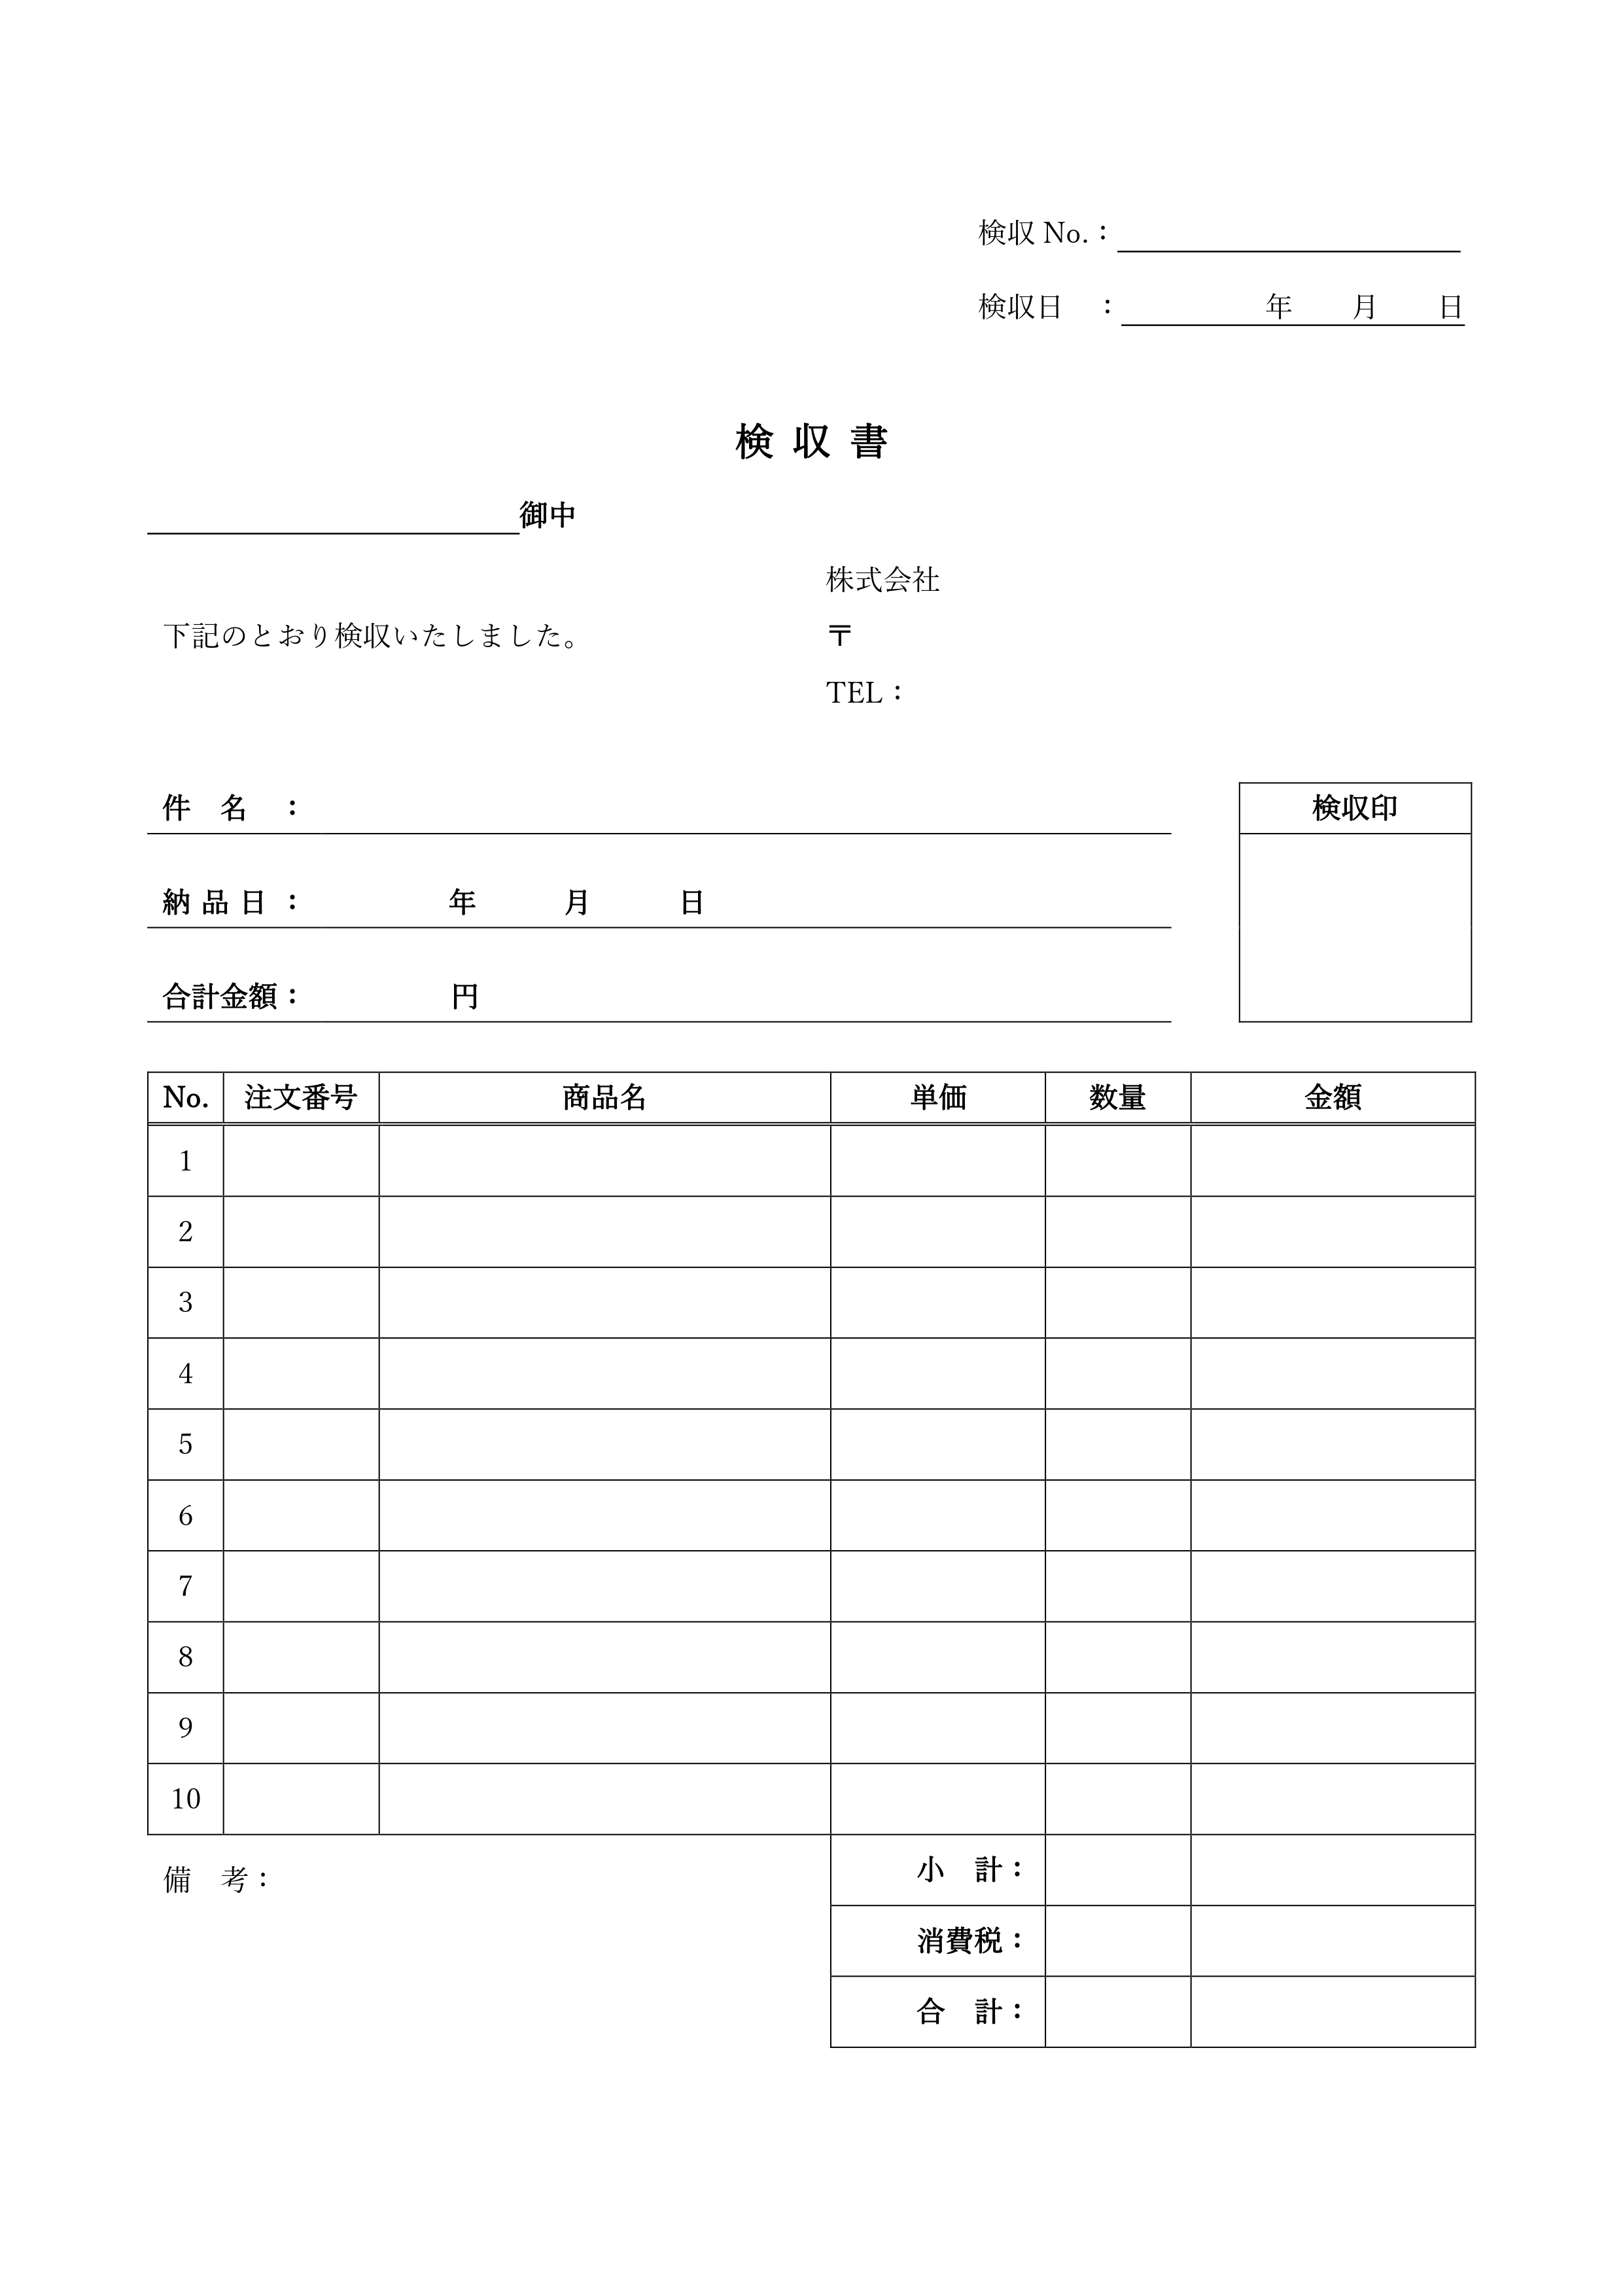
\includegraphics[width=15cm]{image/06-discussion/experiment_A.jpg}
            }
        \caption{実験対象である電子文書の帳票画像A}
        \label{fig:experiment_A}
    \end{center}
\end{figure}

\begin{figure}[tp]
    \begin{center}
        \fbox{
            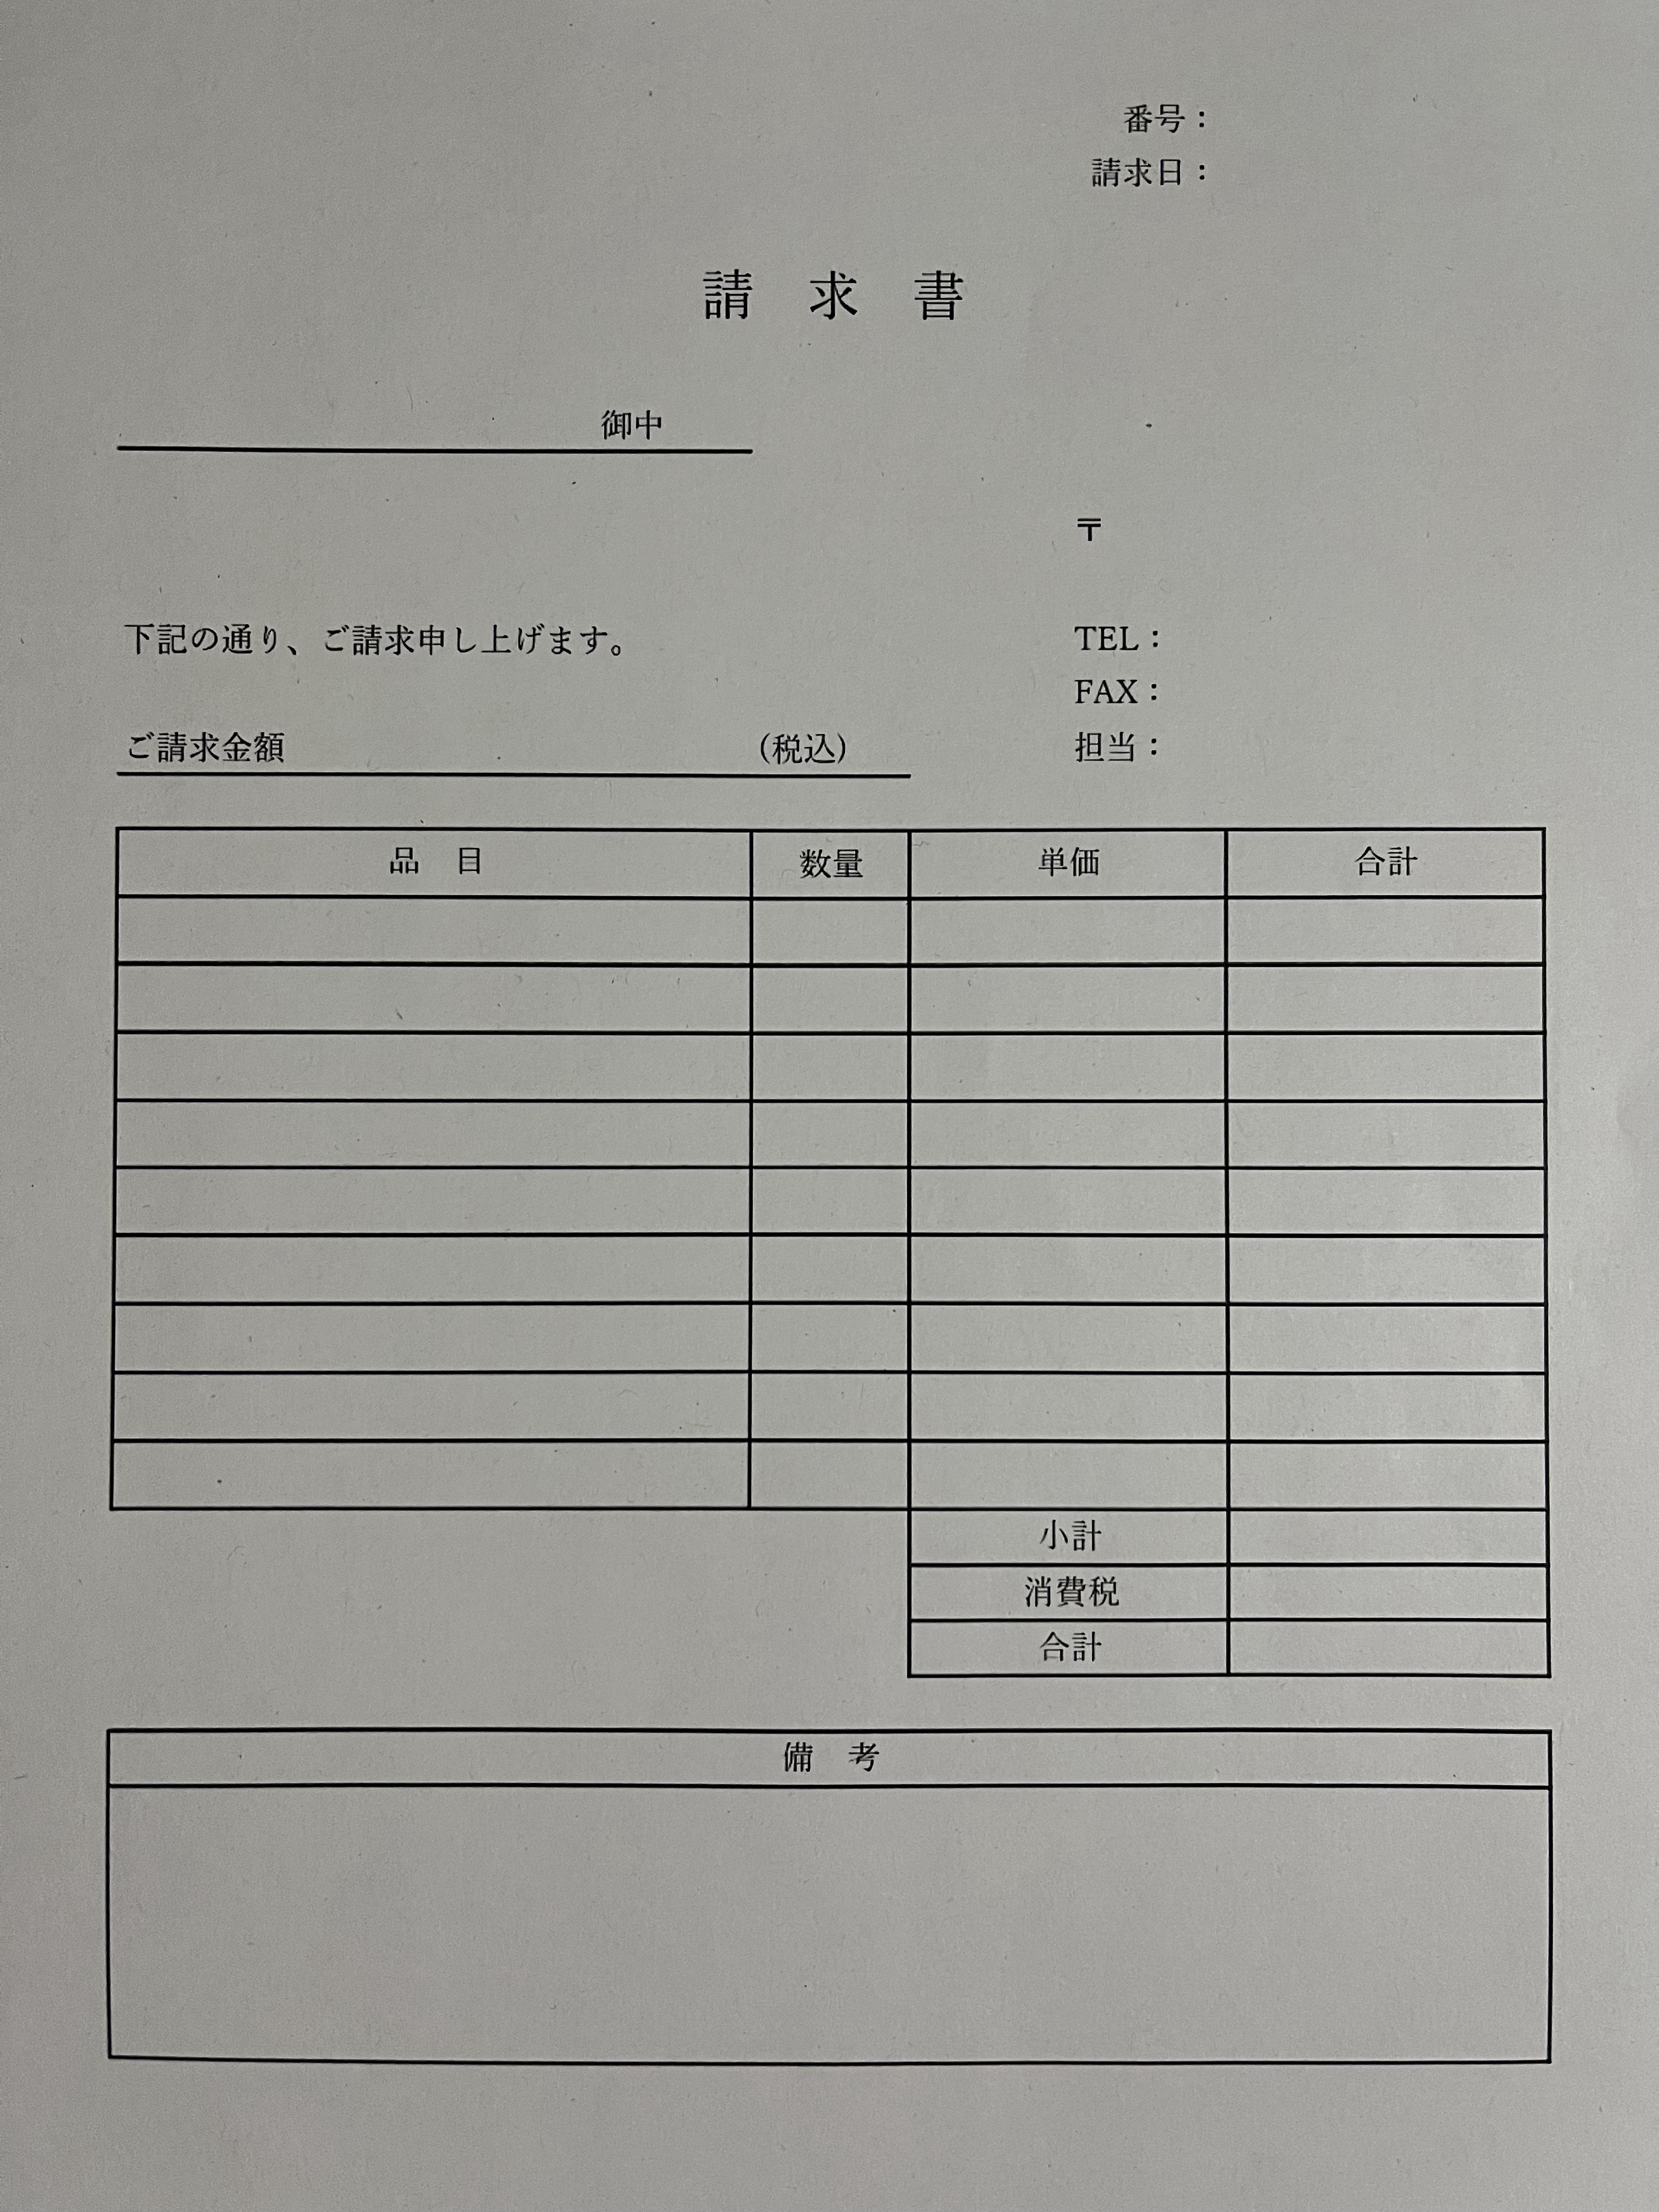
\includegraphics[width=15cm]{image/06-discussion/experiment_B.jpg}
        }
        \caption{実験対象である電子化文書の帳票画像B}
        \label{fig:experiment_B}
    \end{center}
\end{figure}
図\ref{fig:experiment_A}は、電子文書の画像であり、図\ref{fig:experiment_B}は、電子化文書の画像である。
以降、図\ref{fig:experiment_A}の画像を、帳票画像A、図\ref{fig:experiment_B}の画像を、帳票画像Bと呼ぶ。
なお、帳票画像内記入欄の数は、それぞれ図\ref{fig:experiment_A}が54個、図\ref{fig:experiment_B}が48個である。

実験は、宮崎大学工学部情報システム工学科に所属する学部4年生2名、および修士1年生3名、2年生1名の計6名を対象として行った。

実験は、被験者6名をグループ$\alpha$とグループ$\beta$の2グループに分けて行う。
グループ$\alpha$は、図\ref{fig:experiment_A}の帳票画像Aに対して、試作したツールを適用せず、PhotolizeのGUIツールのみを用いて電子フォーム内記入欄を配置する。
次に、図\ref{fig:experiment_B}の帳票画像Bに対して、試作したツールを適用し、必要に応じてPhorolizeのGUIツールを用いて、電子フォーム内記入欄を再配置する。
グループ$\beta$は、図\ref{fig:experiment_A}の帳票画像Aに対して、試作したツールを適用し、必要に応じてPhorolizeのGUIツールを用いて、電子フォーム内記入欄を再配置する。
次に、図\ref{fig:experiment_B}の帳票画像Bに対して、試作したツールを適用せず、PhotolizeのGUIツールのみを用いて電子フォーム内記入欄を配置する。

被験者のグループ分けと実験手法を、表\ref{tb:experiment_case}に示す。
\begin{table}[tp]
	\centering
	\caption{被験者のグループ分けと実験手法}
    \label{tb:experiment_case}
    \begin{tabular}{cc}
        \begin{minipage}[c]{0.45\hsize}
            \centering
            \begin{tabular}{c|c|c}
                グループ & 被験者 & 学年\\
                \hline \hline
                \multirow{3}{*}{グループ$\alpha$} & 被験者1 & 修士2年生\\
                                               & 被験者2 & 修士1年生\\
                                               & 被験者3 & 学部4年生\\
                                        \hline
                \multirow{3}{*}{グループ$\beta$} & 被験者4 & 修士1年生\\
                                              & 被験者5 & 修士1年生\\
                                              & 被験者6 & 学部4年生
	        \end{tabular}
        \end{minipage} &
        \begin{minipage}[c]{0.45\hsize}
            \centering
            \begin{tabular}{c|c|c}
                グループ & 帳票画像 & 手法 \\
                \hline \hline
                \multirow{2}{*}{グループ$\alpha$} & 帳票画像A & GUIツールのみ \\
                                               & 帳票画像B & 試作ツール + 修正 \\
                                        \hline
                \multirow{2}{*}{グループ$\beta$} & 帳票画像A & 試作ツール + 修正 \\
                                              & 帳票画像B & GUIツールのみ
            \end{tabular}
        \end{minipage}
    \end{tabular}
\end{table}
なお、試作したツールで取得した領域座標、および、ラベルについては、間違っている可能性がある。
修正対象とする電子フォーム内記入欄を、以下に示す。

\begin{itemize}
    \item 誤検出によって、帳票画像内記入欄が存在しない場所に配置した電子フォーム内記入欄
    \item 帳票画像内に存在する帳票画像内記入欄を検出できず、配置できていない電子フォーム内記入欄
    \item 本来想定するラベルとは異なるラベルを割り付けた電子フォーム内記入欄
\end{itemize}

実験で計測する時間について、試作したツールを適用し、JSONファイルと2枚の領域強調画像を出力するまでの時間を、実行時間と呼ぶ。
また、電子フォーム内記入欄の配置が完了するまでの時間を、配置時間と呼ぶ。

実験にあたり、PhotolizeのGUIツールを用いて、電子フォーム内記入欄を配置する。
Photolizeの操作画面を、図\ref{fig:photolize}に示す。
\begin{figure}[tp]
    \begin{center}
        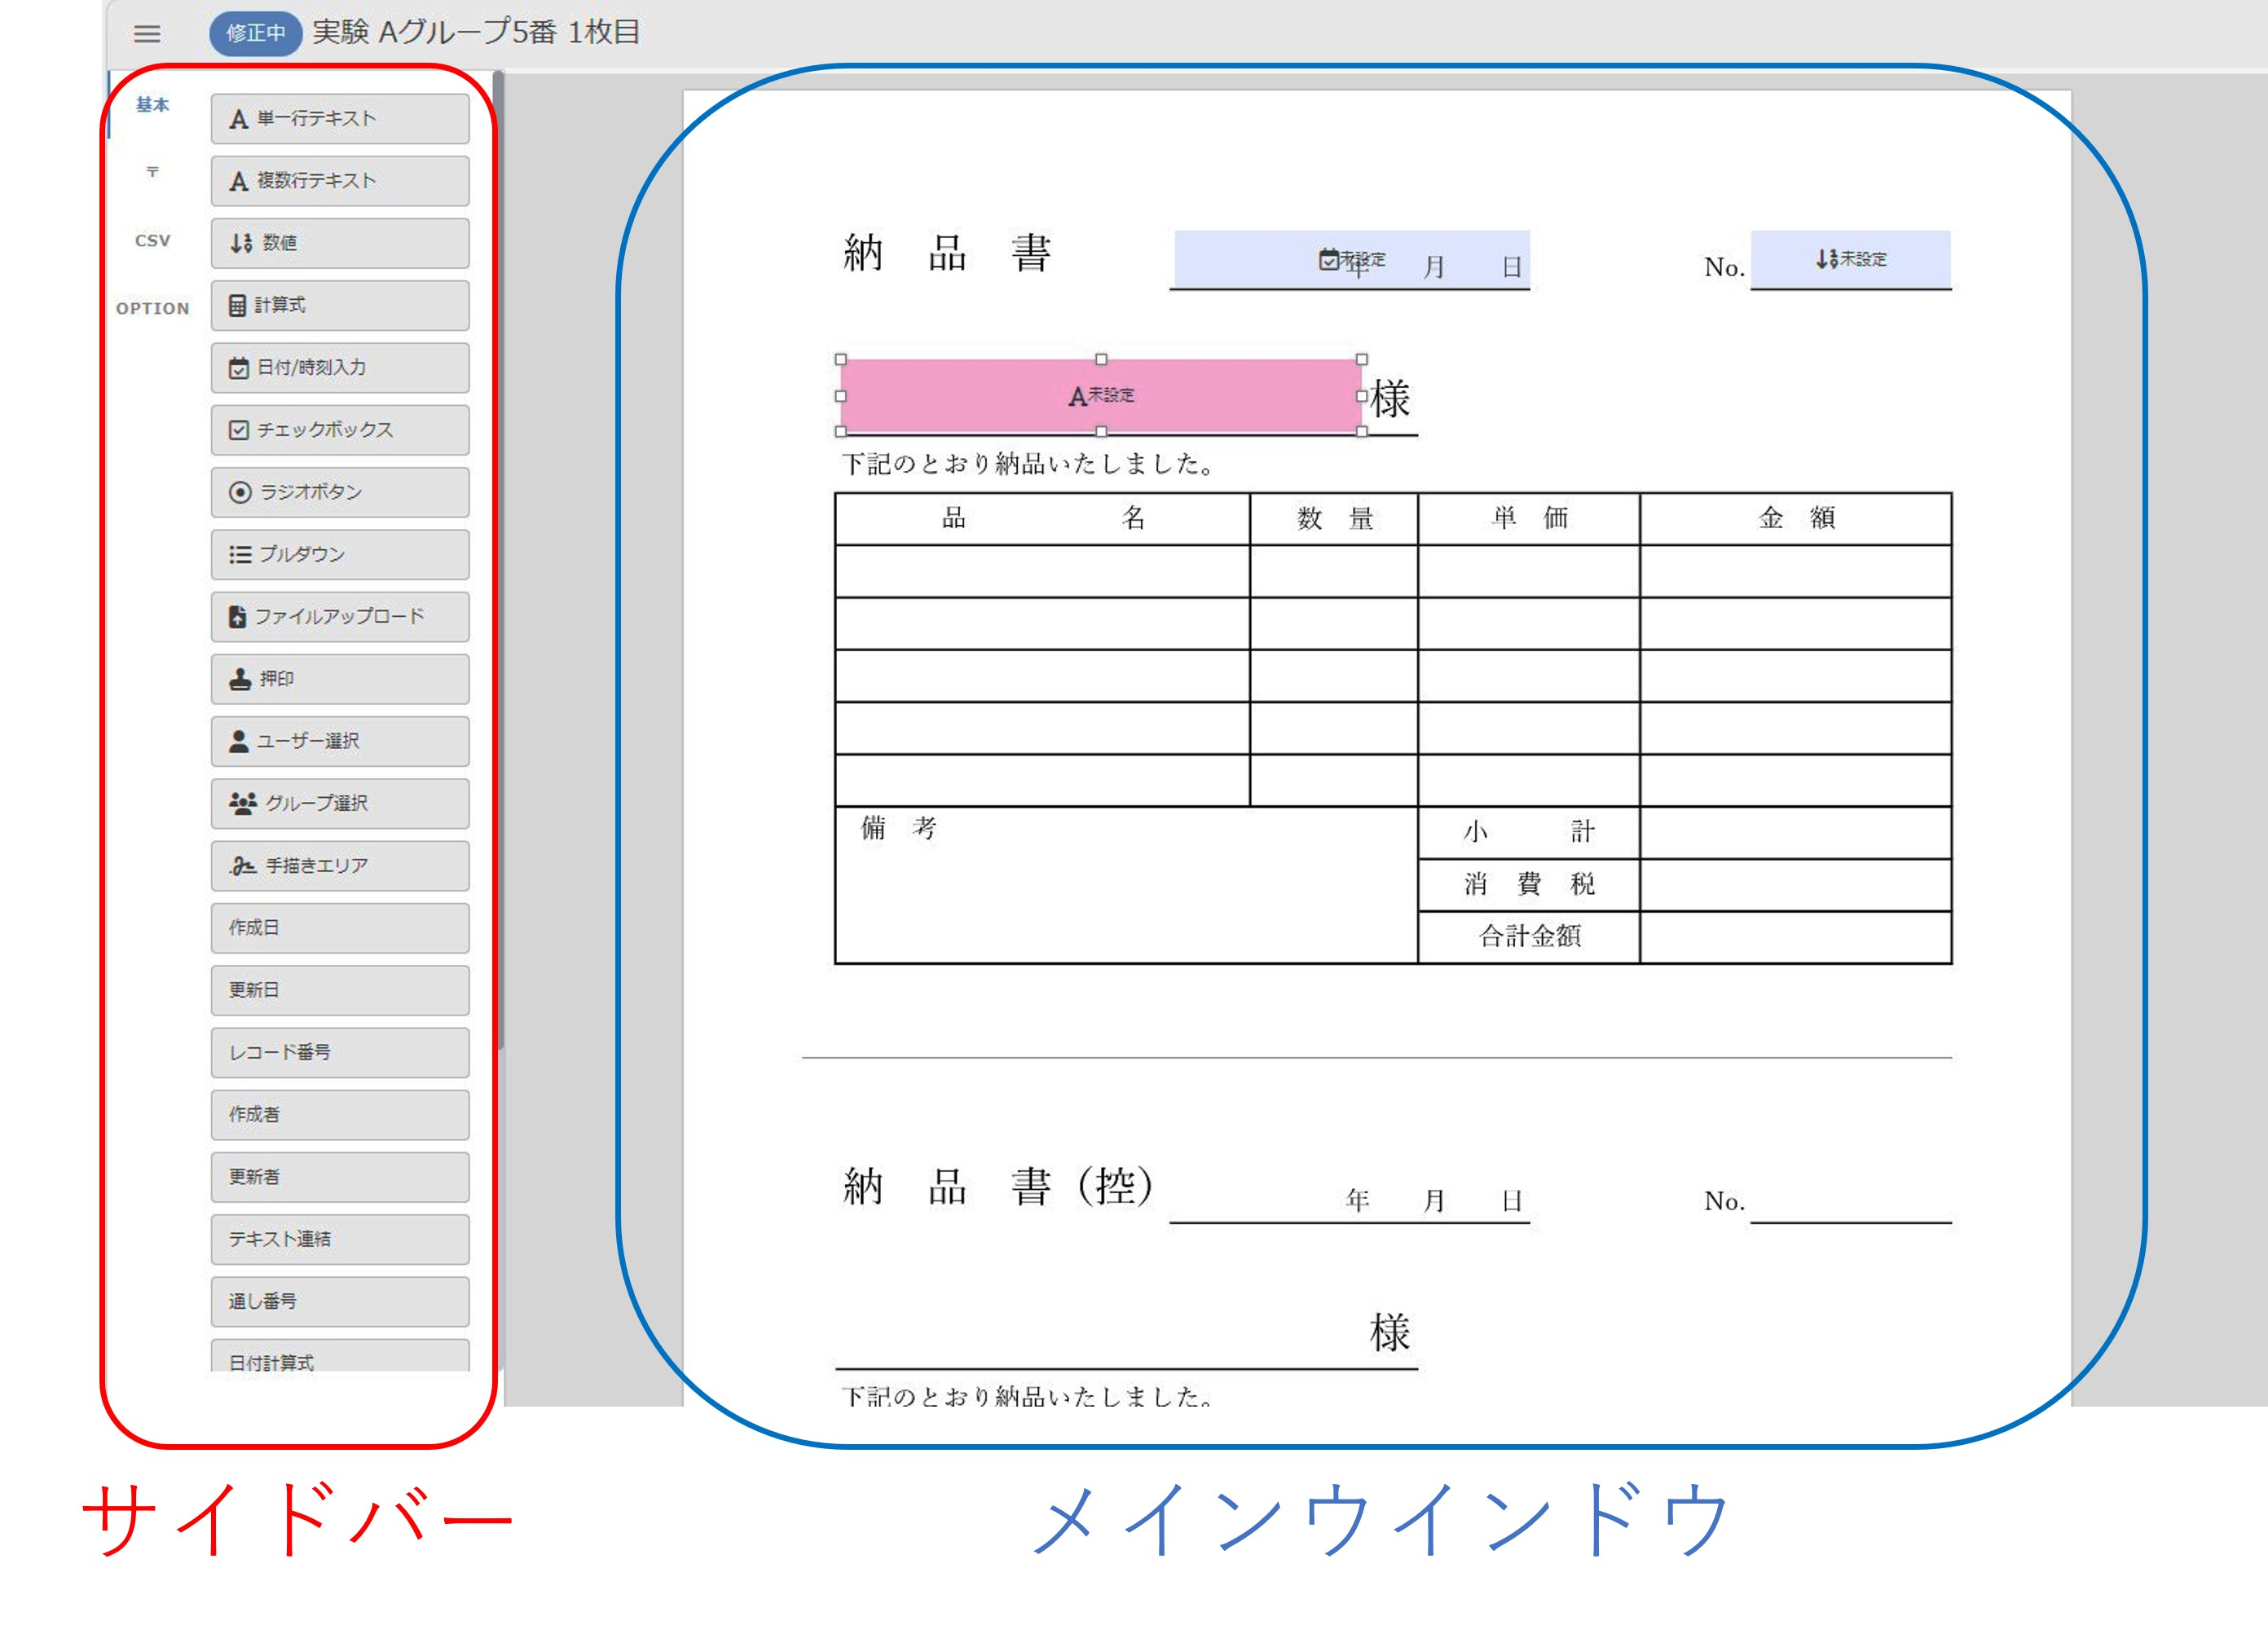
\includegraphics[width=15cm]{image/06-discussion/photolize.jpg}
        \caption{Photolizeの操作画面}
        \label{fig:photolize}
    \end{center}
\end{figure}
Photolizeは、メインウインドウとサイドバーで構成されている。
メインウインドウには、背景とする帳票画像が映される。
配置した電子フォーム内記入欄については青色、配置済みの電子フォーム内記入欄のうち、移動や拡縮などの操作を対象とするものは赤色で表示される。
サイドバーには、配置する電子フォームのラベルの種類を示す複数のボタンがある。
これらのボタンを、メインウインドウの帳票画像上にドラッグすることで、電子フォーム内記入欄を配置する。

PhotolizeのGUIツールを用いて、電子フォーム内記入欄を配置する手順を、図\ref{fig:photolize_how_to_use}に示す。
\begin{figure}[tp]
    \begin{center}
        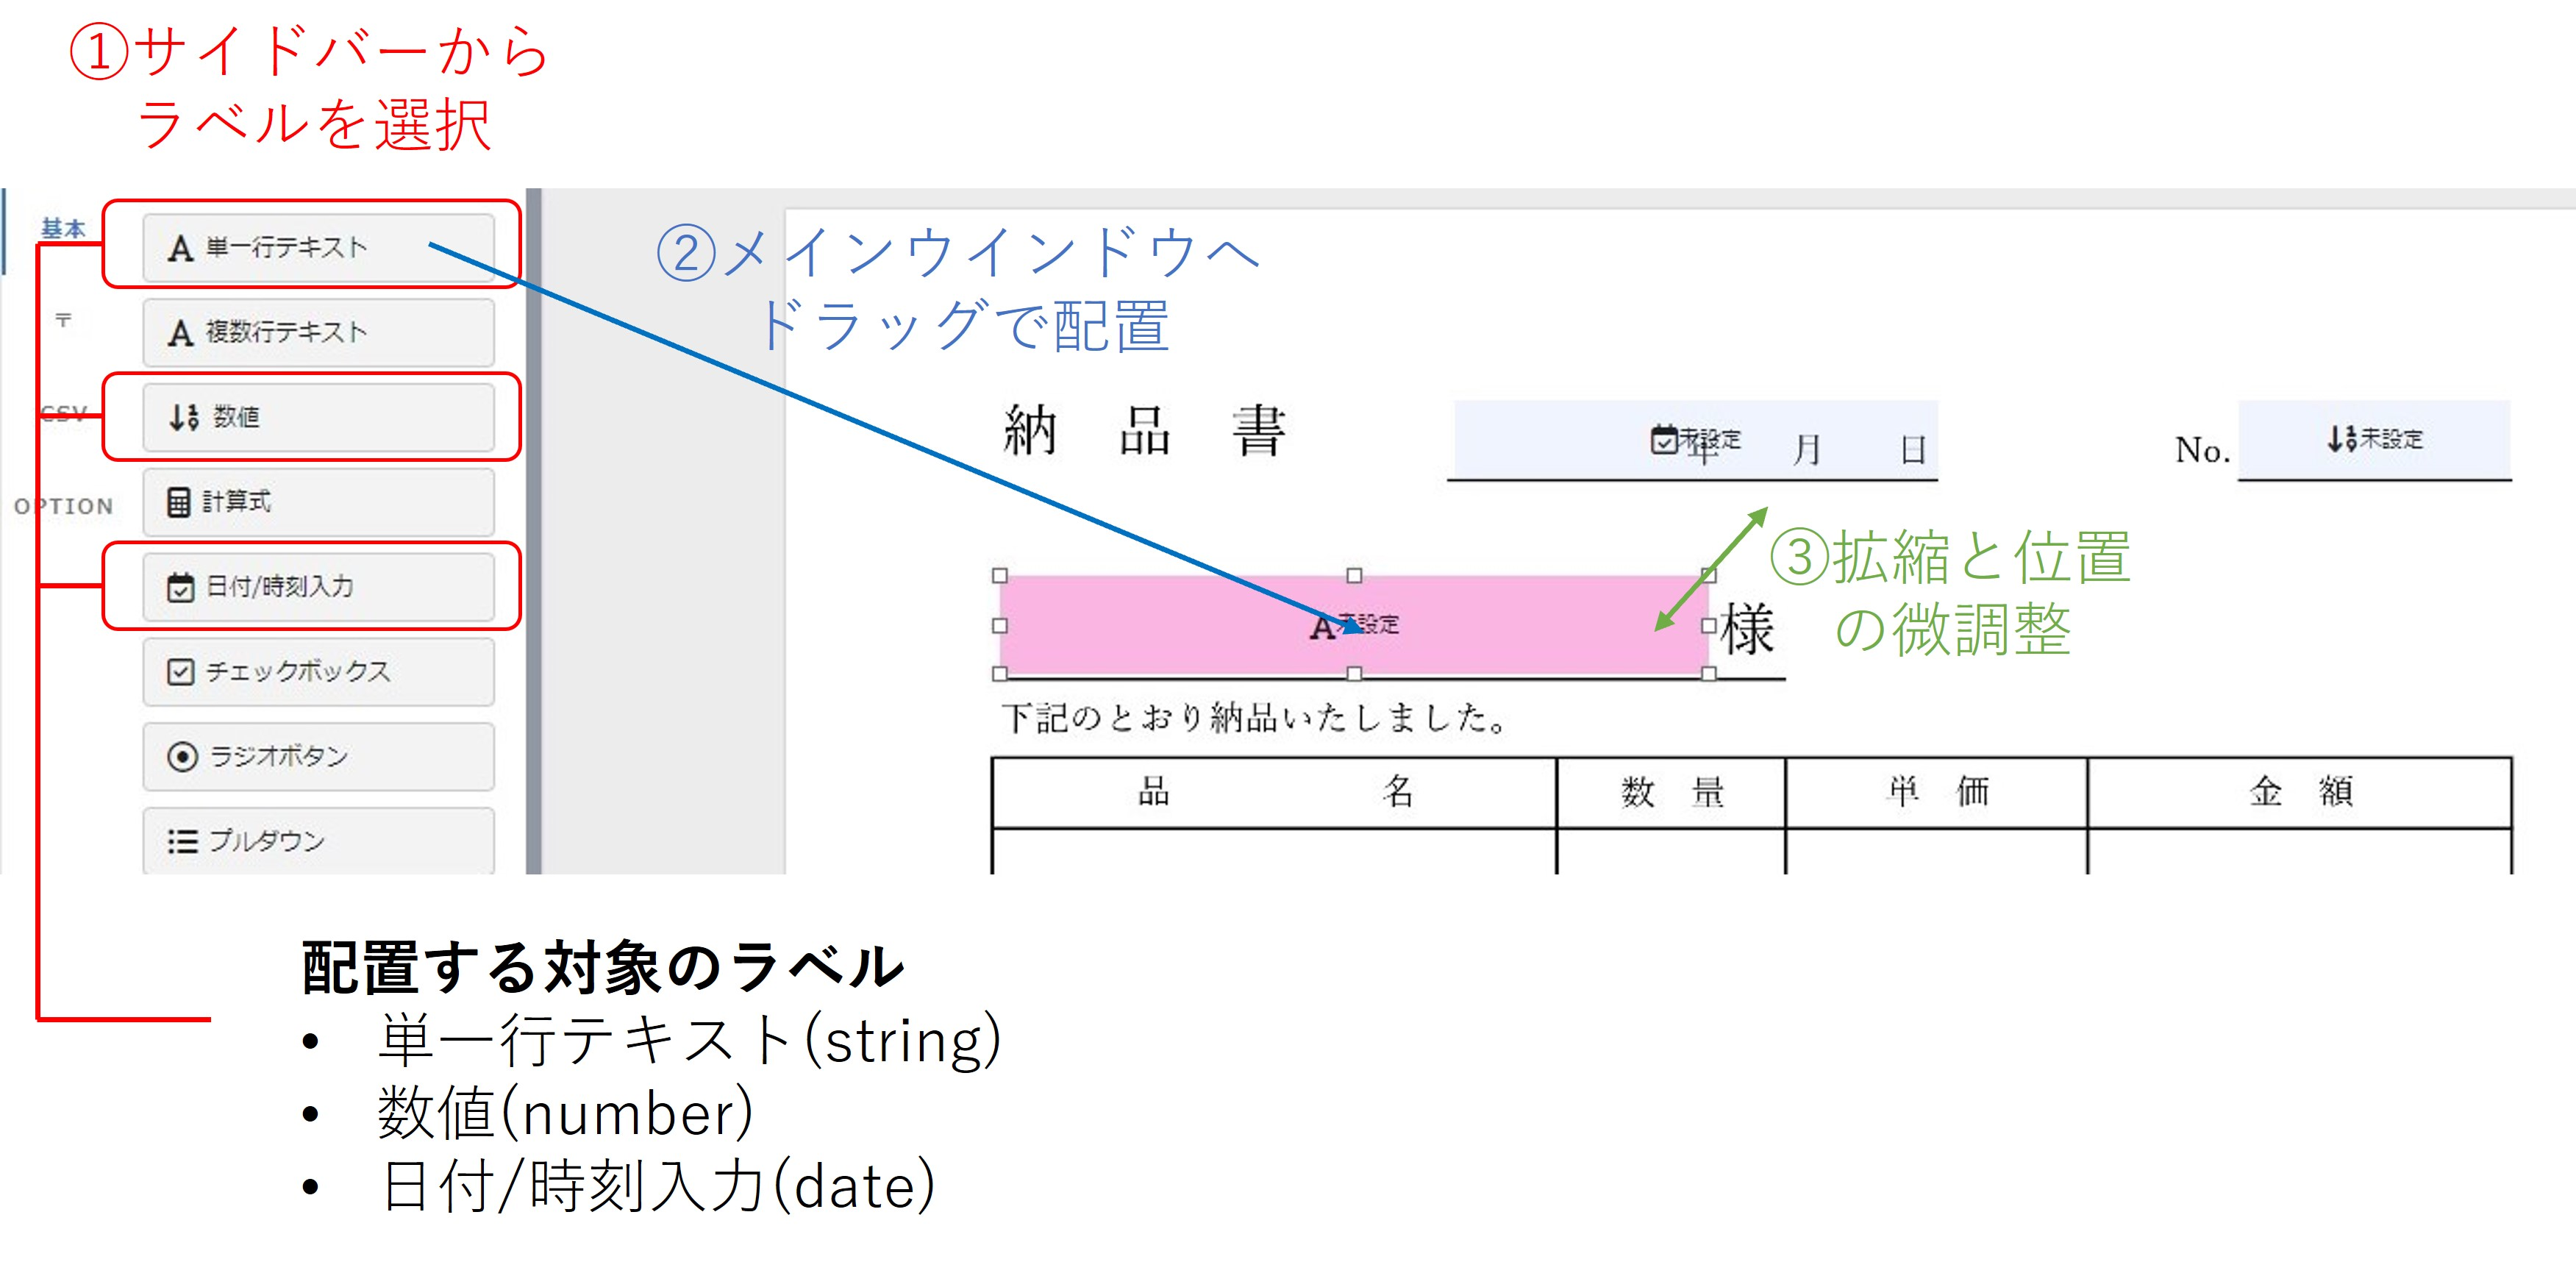
\includegraphics[width=15cm]{image/06-discussion/photolize_how_to_use.jpg}
        \caption{PhotolizeのGUIツールで電子フォーム内記入欄を配置する操作手順}
        \label{fig:photolize_how_to_use}
    \end{center}
\end{figure}
例えば、「個数」を記入する帳票画像内記入欄には、「数値」の電子フォーム内記入欄を選択し、ウインドウに表示する帳票画像内にドラッグすることで、電子フォーム内記入欄を配置できる。
配置した電子フォーム内記入欄については、矩形であり、各頂点と各辺の中点(図\ref{fig:photolize_how_to_use}内の電子フォーム内記入欄上の白い正方形)をドラッグすることで、拡縮を行う。
配置済みの電子フォーム内記入欄のうち、各頂点と各辺の中点でない箇所をドラッグすることで、移動を行う。
なお、Photolizeを利用するにあたり、記入する内容に適する種類の電子フォーム内記入欄を選択して配置することで、ラベルを考慮したとみなす。
今回の実験では、ラベルの種類については、試作したツールにおける日付(date)、文字列(string)、数値(number)に対応するよう、それぞれ「日付/時刻入力」、「単一行テキスト」、「数値」の3種類のみを用いる。

試作したツールを適用し、PhotolizeのGUIツールで電子フォーム内記入欄を配置した結果を修正する場合の実験手順を、以下に示す。

\begin{enumerate}
    \item 実験者は、実行時間を計測を開始し、試作したツールを実行する。
    \item 実験者は、試作したツールがJSONファイルと2枚の画像ファイルを出力したことを確認し、実行時間の計測を終了する。
    \item 実験者は、被験者に対して、実験対象の帳票画像とPhotolizeについて説明し、Photolizeにおける電子フォーム内記入欄の配置操作も併せて説明する。
    \item 実験者は、配置時間の計測を開始し、被験者は、PhotolizeのGUIツールを用いて、試作したツールが配置した電子フォーム内記入欄を確認し、必要があれば修正する。
    \item 実験者は、被験者が全ての電子フォーム内記入欄を正しく配置したことを確認し、配置時間の計測を終了する。
\end{enumerate}

試作したツールを適用せず、PhotolizeのGUIツールのみを用いて、電子フォーム内記入欄を配置する場合の実験手順を、以下に示す。

\begin{enumerate}
    \item 開始前に、実験者が被験者に対して、実験対象の帳票画像とPhotolizeについて説明し、Photolizeにおける電子フォーム内記入欄の配置操作も併せて説明する。
    \item 実験者は、配置時間の計測を開始し、被験者は、PhotolizeのGUIツールのみを用いて、電子フォーム内記入欄を配置する。
    \item 実験者は、被験者が全ての電子フォーム内記入欄を正しく配置したことを確認し、配置時間の計測を終了する。
\end{enumerate}

\subsection{試作したツールが配置した電子フォーム内記入欄の精度に関する考察}\label{subsec:evalue_accuracy}
本節では、試作したツールが配置した電子フォーム内記入欄の精度について、領域座標とラベルについての、それぞれの適合率と再現率を算出し、考察する。

それぞれの適合率、および、再現率を算出する式を、以下に示す。
なお、正しくラベルを割り付けた電子フォーム内記入欄は、配置した電子フォーム内記入欄の位置が正しいことを前提とする。

\begin{equation}\label{eq:area_precision}
    領域座標の適合率=\frac{正しく配置した電子フォーム内記入欄の数}{出力した領域座標の数}
\end{equation}

\begin{equation}\label{eq:area_recall}
    領域座標の再現率=\frac{正しく配置した電子フォーム内記入欄の数}{帳票画像内記入欄の数}
\end{equation}

\begin{equation}\label{eq:label_precision}
    ラベルの適合率=\frac{正しくラベルを割り付けた電子フォーム内記入欄の数}{出力した領域座標の数}
\end{equation}

\begin{equation}\label{eq:label_recall}
    ラベルの再現率=\frac{正しくラベルを割り付けた電子フォーム内記入欄の数}{帳票画像内記入欄の数}
\end{equation}

領域座標の適合率と再現率の平均を、表\ref{tb:result_rect_accuracy}に示す。
また、ラベルの適合率と再現率の平均を、表\ref{tb:result_label_accuracy}に示す。
\begin{table}[tp]
    \centering
    \begin{minipage}[h]{0.47\linewidth}
        \caption{出力した領域座標の適合率と再現率}
        \label{tb:result_rect_accuracy}
        \centering
        \begin{tabular}{r|c|c}
            帳票画像 & 適合率 & 再現率 \\
            \hline \hline
            帳票画像A & 0.806 & 1.000 \\
            帳票画像B & 0.857 & 0.875 \\
        \end{tabular}
    \end{minipage}
    \begin{minipage}[h]{0.47\linewidth}
        \caption{出力したラベルの適合率と再現率}
        \label{tb:result_label_accuracy}
        \centering
        \begin{tabular}{r|c|c}
            帳票画像 & 適合率 & 再現率 \\
            \hline \hline
            帳票画像A & 0.731 & 0.907 \\
            帳票画像B & 0.674 & 0.688 \\
        \end{tabular}
    \end{minipage}
\end{table}
表\ref{tb:result_rect_accuracy}および表\ref{tb:result_label_accuracy}より、2枚の帳票画像に共通して、領域座標およびラベルの再現率は、適合率に比べ高いことがわかる。
式\ref{eq:area_precision}および式\ref{eq:label_precision}より、適合率は、不要に領域座標を取得する回数が少ないほど上昇し、不要に領域座標を取得する回数が多いほど低下する。
また、式\ref{eq:area_recall}および式\ref{eq:label_recall}より、再現率は、正しく配置した電子フォームの数が多いほど上昇し、正しく配置した電子フォームの数が少ないほど低下する。
よって、再現率が高いことから、試作したツールが配置した電子フォーム内記入欄は、配置する必要がある場所については正しく配置できる。
一方、適合率はあまり高くないことから、誤検出が多く、不要な電子フォーム内記入欄を配置していることがわかる。
この結果より、試作したツールを用いて修正する場合は、電子フォーム内記入欄を配置する修正の回数よりも、不要に配置した電子フォーム内記入欄を削除する修正の回数が多いと考察する。

% 電子フォーム内記入欄を配置する場合は、ラベルを考慮しつつ、位置を調整する必要がある。
% 一方、電子フォーム内記入欄を削除する場合は、その必要がないため、電子フォーム内記入欄を配置する場合と比較して、手間がかからない。
% よって、試作したツールは、電子フォーム内記入欄を配置する手間の削減について、有用であることがわかった。

ただし、表\ref{tb:result_rect_accuracy}および表\ref{tb:result_label_accuracy}より、領域座標とラベルについて、領域座標の適合率を除き、帳票画像Bにおける適合率と再現率は、帳票画像Aと比較して低い。
これについては、帳票画像Bに、矩形および下線部で示されていない記入欄を含むことと、帳票画像Bを撮影した環境によって、二値化の結果に影響があり、一部の領域を検知できなかったことが原因であると考察する。
これらの問題については、\ref{sec:problems}節で後述する。

これらの考察を踏まえ、電子フォーム内記入欄を配置するまでにかかった時間を評価する。

\subsection{電子フォーム内記入欄を配置するまでにかかる時間に関する評価}\label{subsec:evalue_required_time}
本節では、電子フォーム内記入欄を配置するまでにかかる時間について、評価を行う。

帳票画像A、Bについて、被験者6名の各計測時間とその合計時間を、表\ref{tb:result_time}に示す。
\begin{table}[tp]
    \caption{被験者が電子フォーム内記入欄を配置するまでにかかる時間(分:秒)}
	\label{tb:result_time}
    \centering
    \begin{tabular}{c|cc||rrr} 
    グループ & 被験者 & 帳票画像 & 実行時間 & 配置時間 & 合計時間 \\
    \hline \hline
    
    \multirow{6}{*}{グループ$\alpha$} & \multirow{2}{*}{被験者1} & 帳票画像A & - & 08:49 & 08:49 \\ % 宮下さん M2  
                                                            & & 帳票画像B & 01:10 & 03:49 & 04:59 \\ 

                                    & \multirow{2}{*}{被験者2} & 帳票画像A & - & 10:03 & 10:03 \\ % 柿木さん M1
                                                            & & 帳票画像B & 01:30 & 02:50 & 04:20 \\
                                                            
                                    & \multirow{2}{*}{被験者3} & 帳票画像A & - & 07:32 & 07:32 \\ % 田中くん B4
                                                            & & 帳票画像B & 01:12 & 03:18 & 04:30 \\
                                                            

                                                            \hline
    \multirow{6}{*}{グループ$\beta$} & \multirow{2}{*}{被験者4} & 帳票画像A & 01:26 & 02:48 & 04:11 \\ % 高倉さん M1
                                                            & & 帳票画像B & - & 07:11 & 07:11 \\
                                                            
                                    & \multirow{2}{*}{被験者5} & 帳票画像A & 01:20 & 02:38 & 03:58 \\ % 翁長さん M1
                                                            & & 帳票画像B & - & 07:32 & 07:32 \\ 
                                                            
                                    & \multirow{2}{*}{被験者6} & 帳票画像A & 01:33 & 02:21 & 03:54 \\
                                                            & & 帳票画像B & - & 06:56 & 06:56 \\ 

    \end{tabular}
\end{table}
また、表\ref{tb:result_time}のうち、帳票画像Aにおける各計測時間の平均を表\ref{tb:result_imageA_mean_time}に、表\ref{tb:result_time}のうち、帳票画像Bにおける各計測時間の平均を表\ref{tb:result_imageB_mean_time}に、それぞれ示す。
\begin{table}[tp]
	\centering
    \begin{tabular}{cc}
        \begin{minipage}[c]{0.5\hsize}
            \centering
            \caption{帳票画像Aにおける各計測時間の平均(分:秒)}
            \label{tb:result_imageA_mean_time}
            \begin{tabular}{c|rrr}
                グループ & 実行時間 & 配置時間 & 合計時間 \\
                \hline \hline
                グループ$\alpha$ & - & 08:48 & 08:48 \\
                グループ$\beta$ & 01:26 & 02:36 & 04:02 \\
	        \end{tabular}
        \end{minipage} &
        \begin{minipage}[c]{0.5\hsize}
            \centering
            \caption{帳票画像Bにおける各計測時間の平均(分:秒)}
            \label{tb:result_imageB_mean_time}
            \begin{tabular}{c|rrr}
                グループ & 実行時間 & 配置時間 & 合計時間 \\
                \hline \hline
                グループ$\alpha$ & 01:12 & 03:19 & 04:31 \\
                グループ$\beta$ & - & 07:13 & 07:13 \\
            \end{tabular}
        \end{minipage}
    \end{tabular}
\end{table}
合計時間を算出する式を、式\ref{eq:sum_time}に示す。
なお、PhotolizeのGUIツールのみを用いて枠を配置した場合は、実行時間は0秒として計算する。

\begin{equation}\label{eq:sum_time}
    合計時間=実行時間+配置時間
\end{equation}

表\ref{tb:result_imageA_mean_time}より、帳票画像Aに関する合計時間は、試作したツールを使用したグループ$\beta$が、PhotolizeのGUIツールのみを用いたグループ$\alpha$よりも平均で4分46秒(約54.17\%)短い。
同様に、表\ref{tb:result_imageB_mean_time}より、帳票画像Bに関する合計時間は、試作したツールを使用したグループ$\alpha$が、PhotolizeのGUIツールのみを用いたグループ$\beta$よりも平均で2分42秒(約37.41\%)短い。
以上の結果から、試作したツールは、電子フォーム内記入欄を配置する時間の削減について、有用であることがわかった。




\section{関連ツール}\label{sec:relation_tools}
本節では、本研究で試作した記入欄自動検出およびラベル割付機能を持つツールと、関連ツールを比較する。
電子フォーム作成ツールに、株式会社シムトップスのi-Reporter\cite{i-Reporter}や、インフォテック株式会社のCreate!Form\cite{Create!Form}がある。
これらの既存の電子フォーム作成ツールは、帳票をExcelファイルとして管理している場合は、電子フォームを簡単かつExcelファイルのレイアウトとセルの書式を保って作成できる。
一方、帳票を紙媒体で管理している場合は、既存の電子フォーム作成ツールを使用するために、帳票をExcelファイルとして作成し、入力とするか、紙媒体の帳票を撮影した画像ファイルを入力として、電子フォームを手作業で作成する必要があり、それぞれ以下の2つの課題がある。

\begin{itemize}
    \item Excelファイルを入力とする場合、紙媒体のレイアウトをもとにExcelファイルを作成する必要があり、使い慣れた既存の帳票のレイアウトが変わる場合がある。
    \item 画像ファイルを入力とする場合、画像を背景として、GUIツールを用いたマウス操作で記入欄を配置する必要があるため、電子フォームの作成に時間がかかる。
  \end{itemize}

また、サイボウズ社が提供するクラウドサービスであるkintone\cite{kintone}を利用し、データベースに保存したデータから、記入済みの帳票を自動作成する外部連携サービスに、トヨクモ社のPrintCreator\cite{PrintCreator}や、オーサムジョブ社のk-Report\cite{k-Report}がある。
しかし、背景となるPDFファイルを用意し、電子フォーム内記入欄をGUIツールのマウス操作で配置することによって、帳票のテンプレートを作成する必要があり、時間がかかる。
このように、既存の電子フォーム作成ツールやサービスは、これらの課題を同時に解決できない。

試作したツールは、レイアウトを保持したまま、帳票画像内記入欄を自動検出し、バリデーションチェックに必要である記入内容のデータ型をラベルとして割り付け、JSONファイルとして出力できる。
また、JSONファイルの内容を人間が確認しやすくするため、自動検出した帳票画像内記入欄と、そのラベルを強調表示して、画像として出力できる。
これにより、試作したツールを適用することによって、レイアウトを保持したまま、電子フォーム作成にかかる時間を削減できる。

\section{試作したツールの問題点}\label{sec:problems}
試作したツールの問題点を、以下に示す。

\begin{itemize}
    \item 記入内容を示す欄を、帳票画像内記入欄として検出する\\
        矩形領域と下線部領域は、それぞれ矩形と直線を検出し、領域座標を取得したものである。
        領域座標取得部(\ref{sec:area_coords_obtainment_part}節を参照)において、文字情報を参照しないため、取得した領域座標が記入する内容を示す欄か、もしくは、帳票画像内記入欄かを判別できない。
        特に、矩形が隣接する形式の帳票である際、行または列が記入する内容を示す場合がある。
        これによって、記入する内容を示す欄の数だけ、不要に領域座標を出力してしまう。
        この問題点については、取得した領域座標と文字位置を参照し、領域座標の中心点から一定の範囲内であれば、出力から除外することで解決できると考える。
    \item 割り付けるラベルが不安定である\\
        試作したツールにおいて、割り付けるラベルは、文字情報とYouriの出力に依存する。
        Tesseract-OCRは、光学文字認識の結果が必ずしも正しいとは限らず、本来認識するべき文字とは別の文字として認識する場合がある。
        例えば、「は」と「ば」などの視覚的な違いが少ない文字や、「品」と「口」などの一部に別の漢字を含む漢字が存在する場合は、誤認識する可能性が高い。
        この誤認識によって、\ref{sec:result_rect}節で述べたような、誤ったラベルを割り付ける場合がある。
        また、Youriの出力は、誤って属性を推測する場合があり、かつ出力が常に一定ではない。
        Tesseract-OCRとYouriの2つの不安定な出力によって決定するため、割り付けるラベルも不安定となる。
        この問題点については、他の光学文字認識ソフトウェアの利用や、プロンプトの改善によって解決できると考える。
    \item 特殊なレイアウトの帳票画像においては、精度が低下する\\
        欄の一部に色が付いているもの、絵や押印を含むものなど、記入欄と文字以外のものが帳票画像にある場合は、領域座標を取得する精度と、ラベルを割り付ける精度の両方が低下する。
        これは、帳票画像内記入欄、二値化の結果に影響を及ぼすためである。
        特に、青や紫などの暗色は、グレースケール画像において画素値が高くなり、二値化した際に黒となる可能性が高い。
        二値化によって、記入欄と文字以外に黒の画素が存在する場合、誤検出の可能性が高くなる。
        この問題点については、二値化手法の変更や、一定範囲内に閾値を超える数の黒の画素を認識した場合は、隣接する黒色の画素を白色に変換することで解決できると考える。
    \item 記入内容を示す文字が帳票画像内記入欄の右にある場合は、他の文字の属性をラベルとして割り付けてしまう\\
        ラベル割付処理(\ref{subsec:label_link_processing}節を参照)で述べたラベルを割り付ける手法は、記入内容を示す文字が帳票画像内記入欄の左にある場合のみに正常に動作する。
        記入内容を示す文字が帳票画像内記入欄の右にある場合もラベルの更新を行った場合、行ごとに共通したラベルを割り付けてしまうため、1列ごとに記入内容を決定する形式の帳票に対しては、正常にラベルを割り付けることができない。
        この問題点については、帳票の記入方向を検知し、検知した結果によってラベルを更新する順番を変更することで解決できると考える。
    \item 記入欄の一部が、矩形または下線部で表示されていない場合は、領域座標を取得できない\\
        帳票画像内記入欄は、矩形または下線部で示されていることを前提とするため、文字のみで帳票画像内記入欄を示すものについては、領域座標を取得できない。
        この問題点については、光学文字認識の結果、品詞が名詞である単語のみを認識した場合は、その単語のバウンディングボックスと同じ矩形を右に配置することで解決できると考える。
    \item 撮影環境によって、矩形と下線部の検出、および文字認識の精度が低下する\\
        図\ref{fig:experiment_B}のような電子化文書の画像を入力とした場合は、電子文書の画像と比較して、矩形と下線部の検出、および文字認識の精度が低い傾向にある。
        これは、DeblurGANv2で除去できなかったブレや、撮影場所の明るさ、撮影時に映る影などの撮影環境が二値化の結果に影響を及ぼすためである。
        この問題点については、陰影除去などの別の画像処理を加えることで解決できると考える。
\end{itemize}